\documentclass[
    aspectratio=1610
    ]{beamer}
\usepackage{chemfig}
\usepackage{url}
\usepackage[german]{babel}

\graphicspath{/figures}

\renewcommand\printatom[1]{\ensuremath{\mathsf{#1}}}
\newcommand\namebond[5][-1pt]{\chemmove{\path(#2)--(#3)node[midway,#4,yshift=#1,black!60]{#5};}}

\newcommand\arcbetweennodes[3]{
\pgfmathanglebetweenpoints{\pgfpointanchor{#1}{center}}{\pgfpointanchor{#2}{center}}
\let#3\pgfmathresult}

\newcommand\arclabel[6][red]{
\chemmove{
\arcbetweennodes{#4}{#3}\anglestart \arcbetweennodes{#4}{#5}\angleend \draw[#1]([shift=(\anglestart:#2)]#4)arc(\anglestart:\angleend:#2); \pgfmathparse{(\anglestart+\angleend)/2}\let\anglestart\pgfmathresult \node[shift=(\anglestart:#2+1pt)#4,anchor=\anglestart+180,inner sep=0pt,
outer sep=0pt]at(#4){#6};
    }
}

\usetheme[progressbar=frametitle]{metropolis}

\title{Das Haber-Bosch-Verfahren}
\date{20. April 2023}
\author{Julian Galluzzo}
\institute{Leistungskurs Chemie J1, Königin Olga-Stift Gymnasium}

\definecolor{d_blue}{HTML}{004567}
\setbeamercolor{frametitle}{bg=d_blue}

\begin{document}

    \begin{frame}
        \begin{minipage}{11cm}\hspace{-2.5cm}
            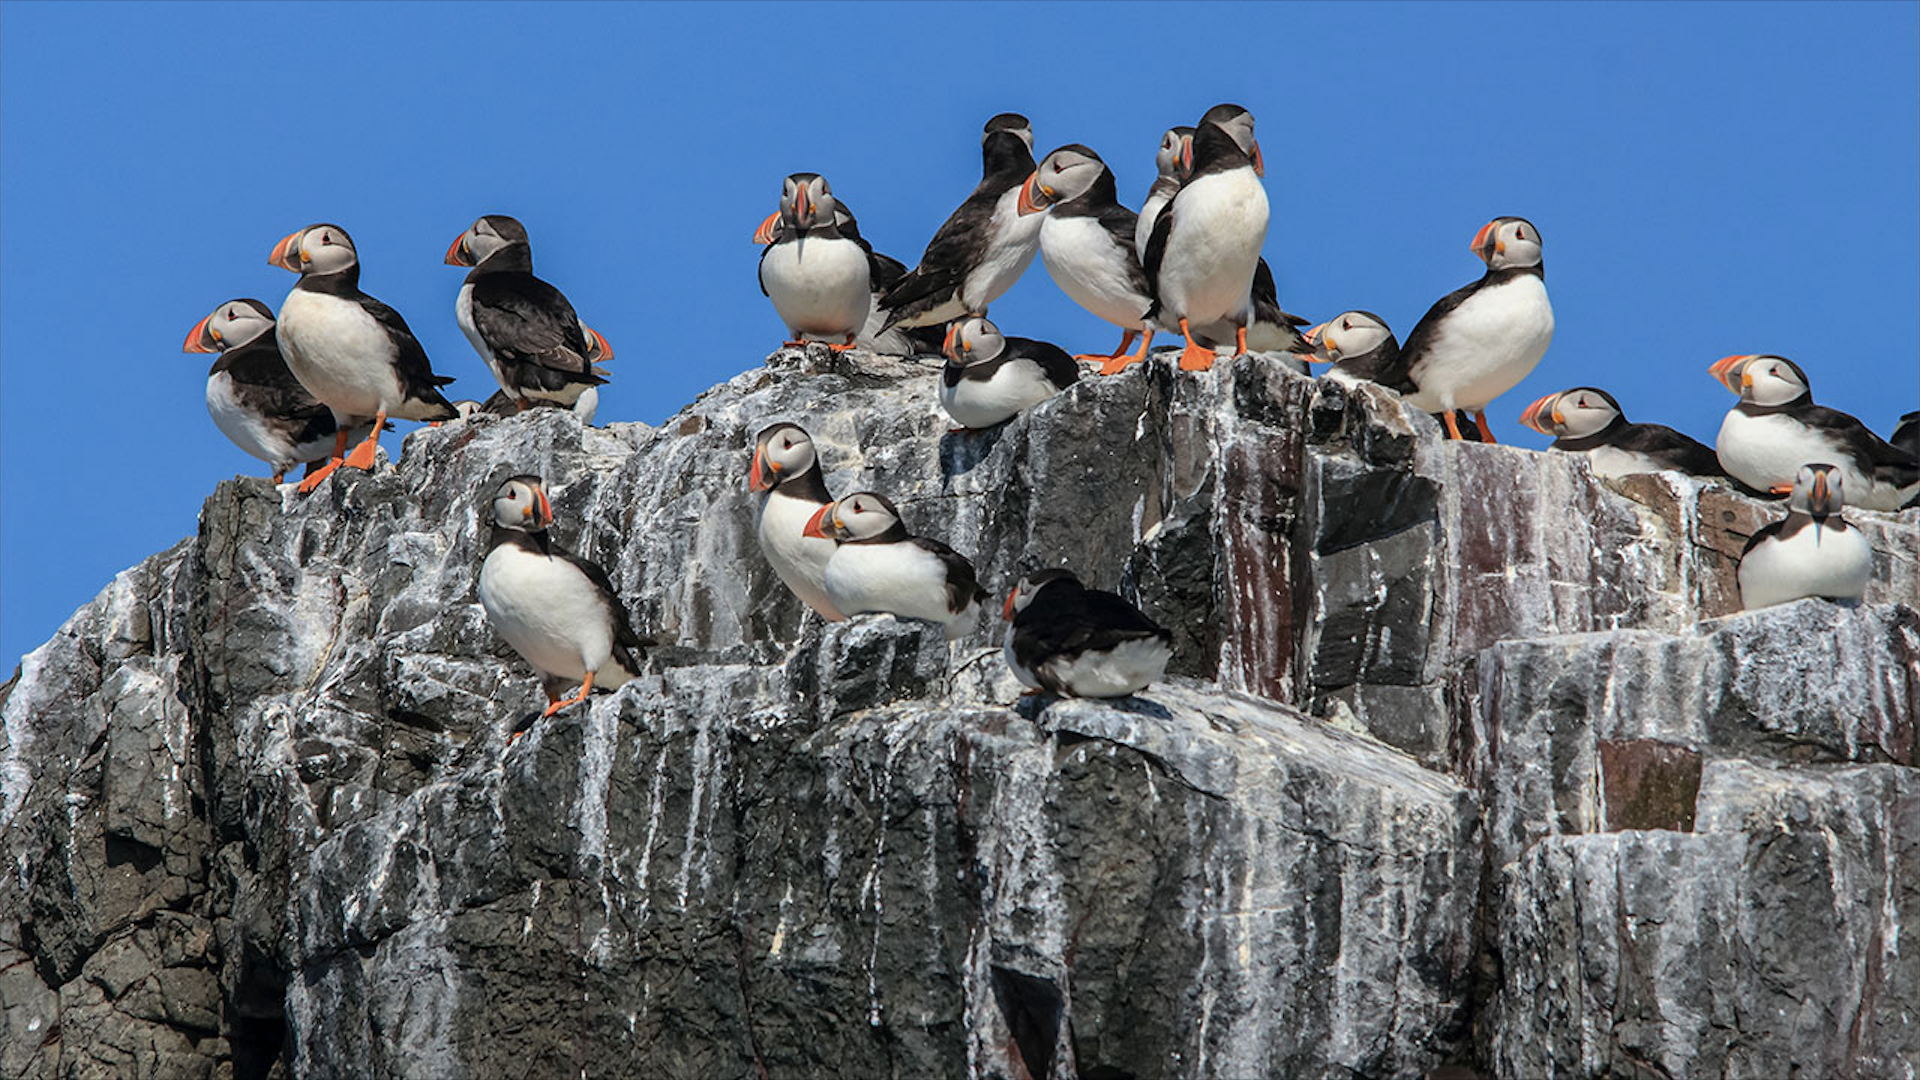
\includegraphics[scale=.3]{figures/GuanoPuffins.png}
        \end{minipage}
    \end{frame}

    \maketitle

    \begin{frame}{Gliederung} 
        \setbeamertemplate{section in toc}[sections not numbered]
        \begin{minipage}{6.75cm}
            \tableofcontents    
        \end{minipage}
        \begin{minipage}{1cm}
            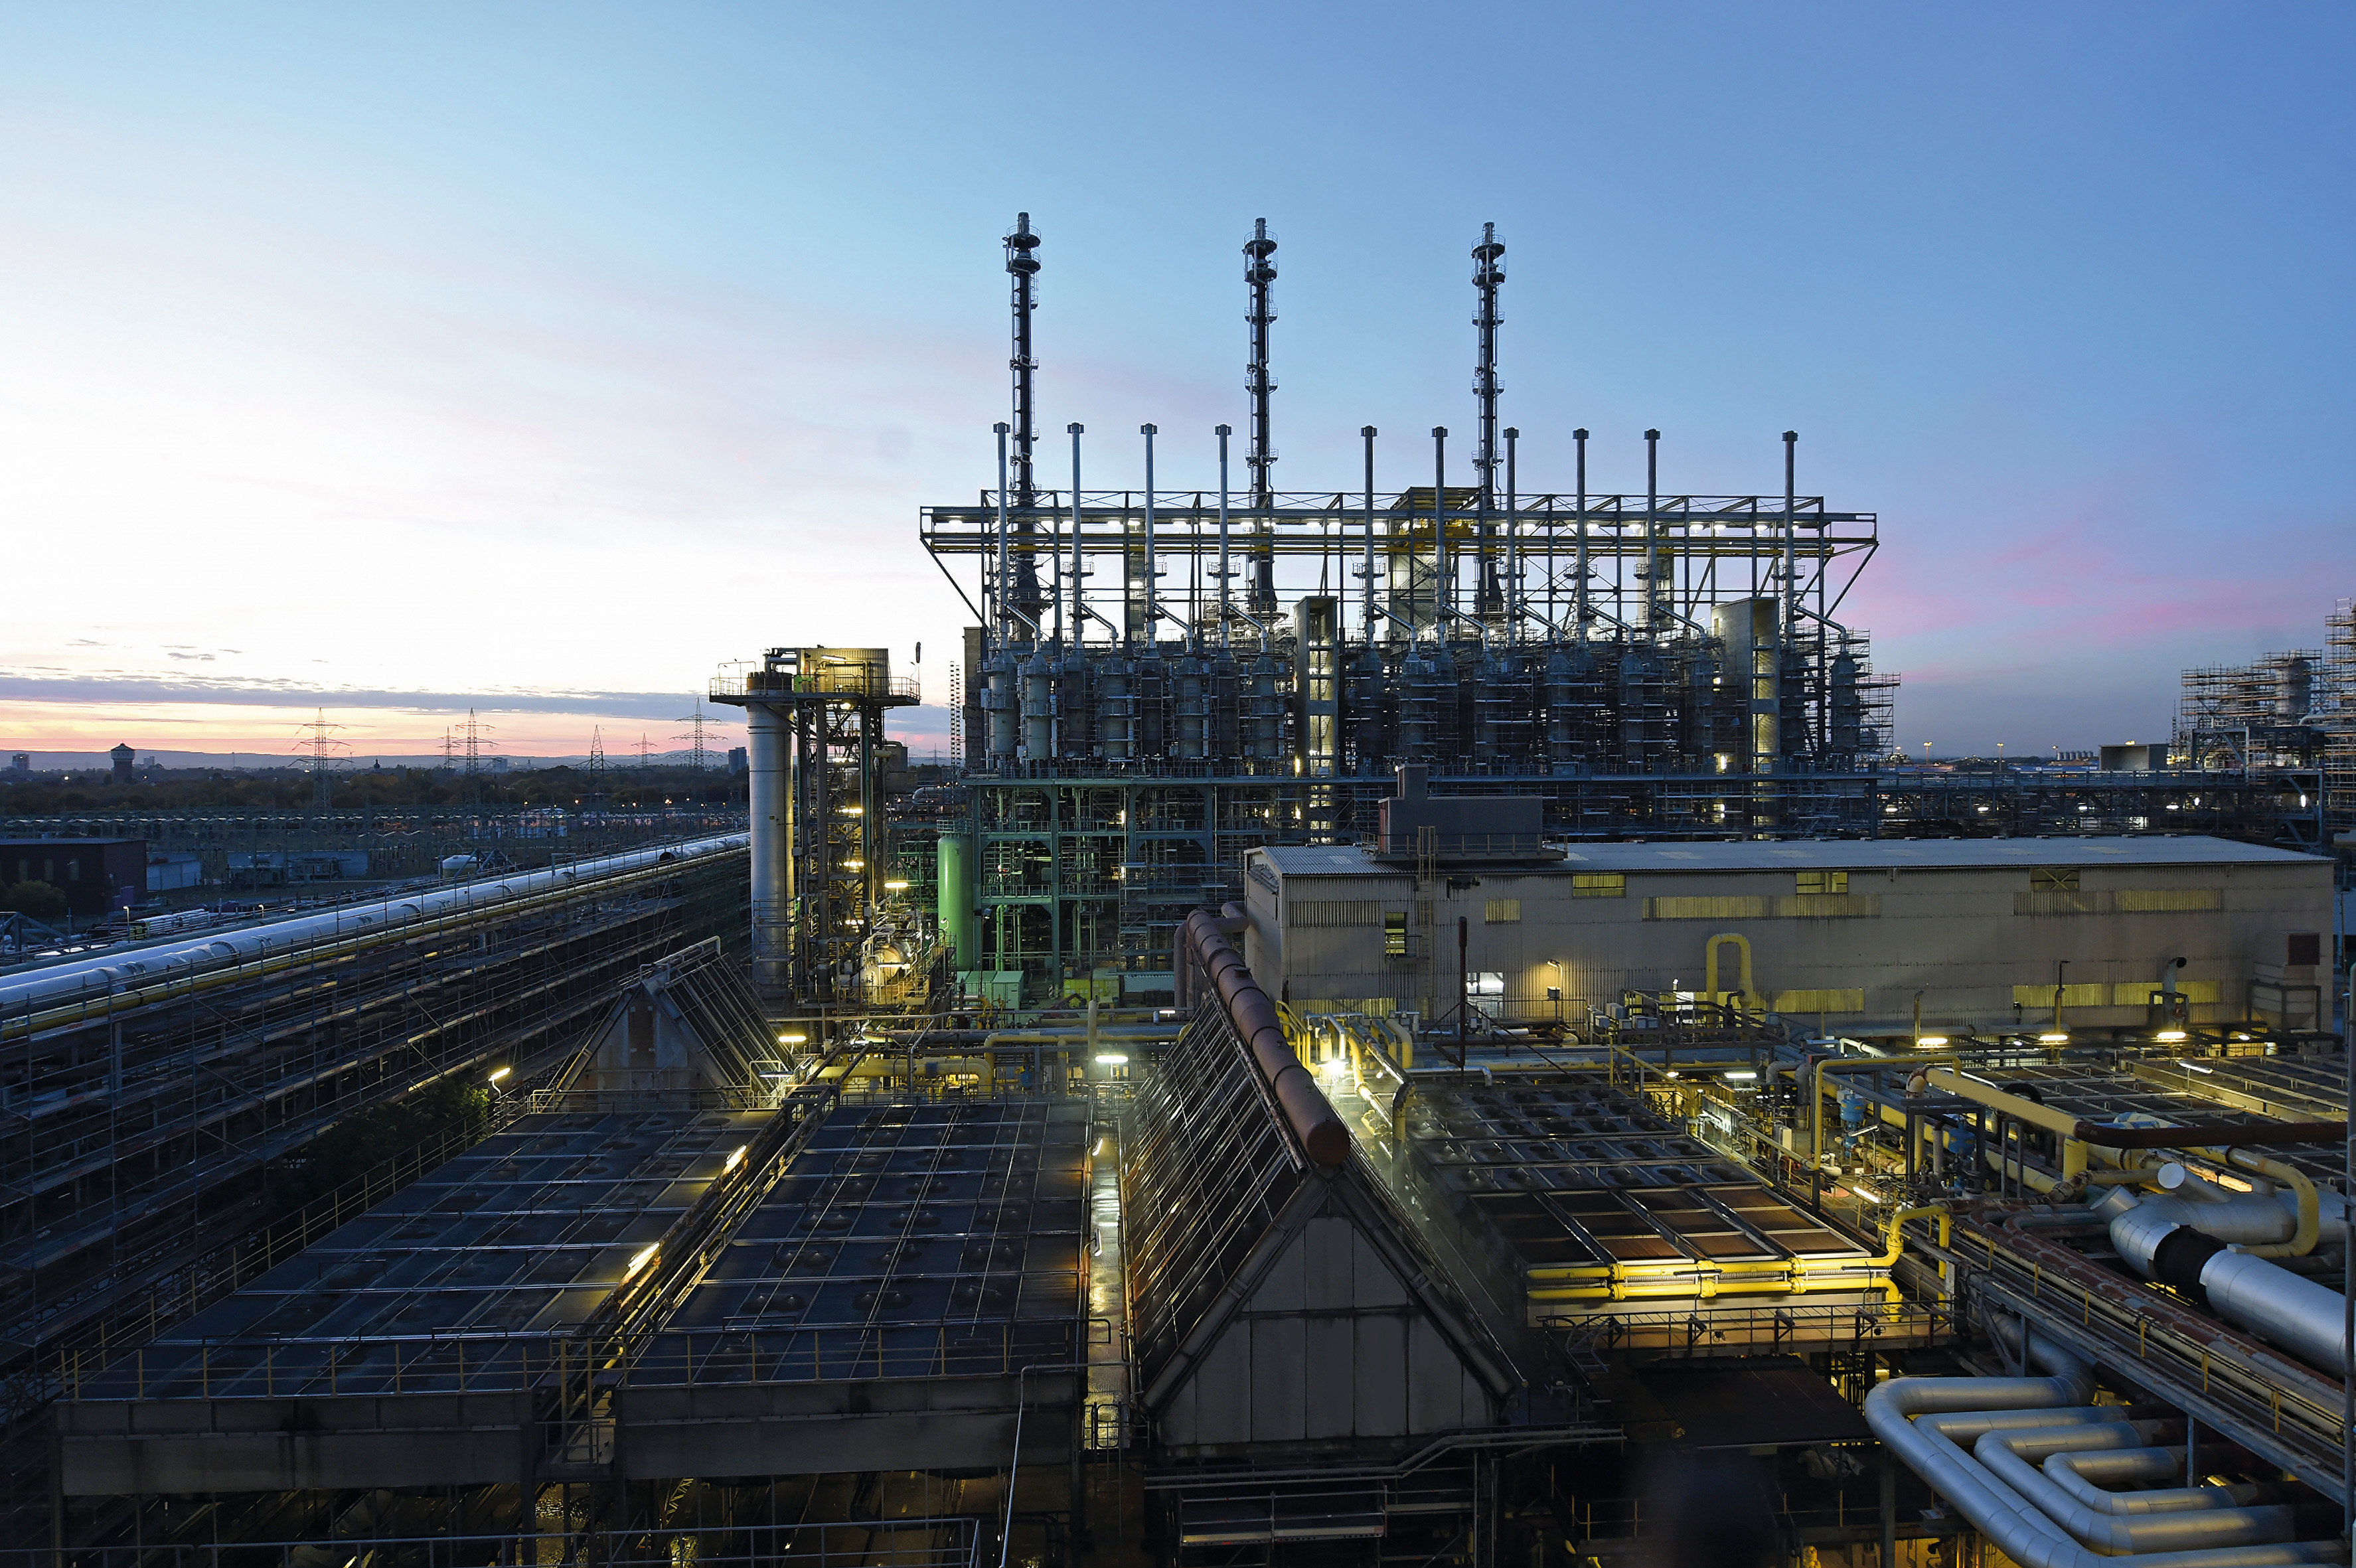
\includegraphics[scale=.25]{figures/Pressefotos.jpg}
            \tiny
        \end{minipage}
    \end{frame}

    \section{\textbf{1.} Was ist Ammoniak?}
    
    \begin{frame}{1. Was ist Ammoniak?}
        \begin{minipage}{8cm}
            \textbf{Chemische Eigenschaften}
            \begin{itemize}
                \item ein alkalischer, anorganischer Stoff 
                \item farblos und hat einen stechenden Geruch
                \item Summenformel: $NH_3$
                \item gehört zur Stoffgruppe der Azane
                \item Schmelztemperatur: -77,73°C
                \newline Siedetemperatur: -33,34°C
                \item hat eine pyramidale Molekülstruktur
                \begin{itemize}
                    \item[$\rightarrow$] Bindungswinkel \alert{$\varphi$ = 106,8°}
                \end{itemize}
            \end{itemize}
        \end{minipage}
        \begin{minipage}{1cm}
            \chemfig[
                atom style={scale=2}
                ]{@{h1}H-[:30]@{n1}{\color{d_blue}{N}}(<:[:-25]H)<[:-57]@{h2}H}
                \color{orange}{
                    \arclabel[scale=3]{0.5cm}{h1}{n1}{h2}{\LARGE\color{black}{\color{orange}$\varphi$}}
                    }
        \end{minipage}
    \end{frame}

    \begin{frame}{1. Was ist Ammoniak?}
        \begin{minipage}{4.35cm}
            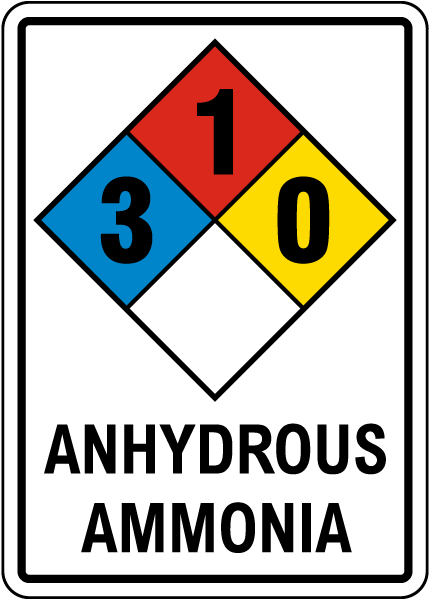
\includegraphics[scale=.25]{figures/NFPA_Anhydrous_Ammonia.png}
            \tiny\url{https://www.safetysign.com/products/14077/nfpa-anhydrous-ammonia-3-1-0-sign}
        \end{minipage}
        \begin{minipage}{9.5cm}
            \textbf{Allgemeine Informationen}
            \begin{itemize}
                \item sehr gut wasserlöslich                
                \item schädlicher Stoff
                \item heute eins der weltweit meistproduzierten Chemikalien (ca. 150 Mio. Tonnen pro Jahr)
                \item[\alert{$\rightarrow$}] \alert{Warum und wie stellen wir so viel Ammoniak her?}
            \end{itemize}
        \end{minipage}        
    \end{frame}
    
    \section{\textbf{2.} Die Bedeutsamkeit des Stickstoffs}
    
    \subsection{\textbf{2.1} Warum ist Stickstoff so wichtig?}
    
    \begin{frame}{2.1 Warum ist Stickstoff so wichtig?}
        \begin{minipage}{6.5cm}
            \vspace{.5cm}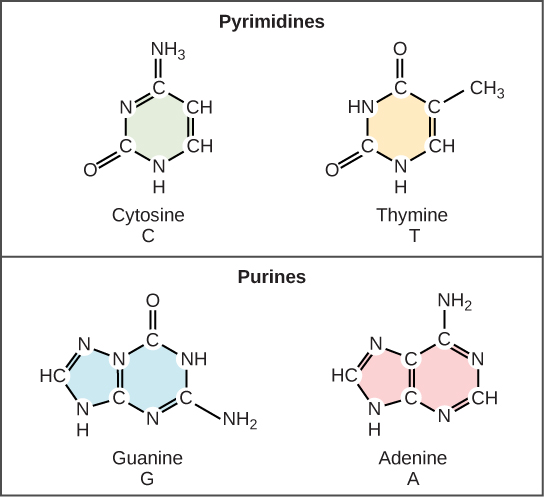
\includegraphics[scale=.7]{figures/DNA_BASES.jpg}
            \color{gray}\tiny\url{https://opentextbc.ca/biology/chapter/9-1-the-structure-of-dna/}
        \end{minipage}
        \begin{minipage}{7cm}
            \begin{itemize}
                \item Stickstoff ist ein wichtiger Bestandteil aller Lebewesen:
                \begin{itemize}
                    \item[$\rightarrow$] Proteine (wichtiger Bestandteil der Aminosäuren)
                    \item[$\rightarrow$] bei Pflanzen, z.B. Chlorophyll
                    \item[$\rightarrow$] Nukleinsäuren (DNA und RNA)
                \end{itemize}
                \item ebenfalls für Sprengstoffe eingesetzt, z.B. bei Kalium- und Natriumnitrat
                \item[\alert{$\rightarrow$}]\alert{vor der synthetischen Herstellung, musste Stickstoff für das Düngen von Pflanzen in der Natur gesucht werden...}
            \end{itemize} 
        \end{minipage}
    \end{frame}
    
    \subsection{\textbf{2.2} Die pazifische Guano-Inseln}

    \begin{frame}{2.2 Die pazifische Guano-Inseln}    
        \begin{minipage}{9.5cm}
            \textbf{Was ist Guano?}
            \begin{itemize}
                \item ein feinkörniges Pulver
                \item entsteht über Jahrtausende bei der Ablagerung von Exkrementen von Seevögeln
                \item enthält bis zu 20\% verwendbare Stickstoffmoleküle für Pflanzen
            \end{itemize}
            \textbf{Die Guano-Inseln}
            \begin{itemize}
                \item Menschen erklärten Vogelinseln in der Pazifik als Privateigentum
                \item ``Guano Islands Act'' im Jahr 1856 verabschiedet (und bis heute noch in Kraft)
            \end{itemize}
        \end{minipage}
        \hspace{.25cm}
        \begin{minipage}{3.5cm}
            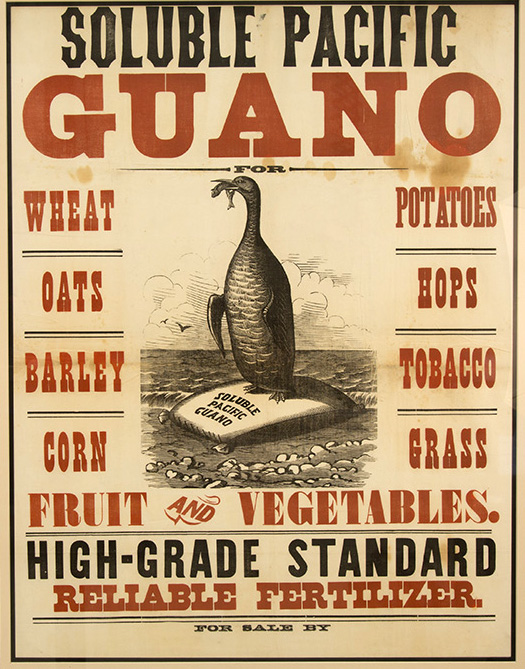
\includegraphics[scale=.3]{figures/GuanoMania.jpg}
            \tiny\color{gray}\url{https://99percentinvisible.org/episode/guano-mania/}
        \end{minipage}
    \end{frame}

    \section{\textbf{3.} Der begrenzte Düngervorrat}
    
    \begin{frame}{3. Der begrenzte Düngervorrat}
        \begin{center}
                \vspace{.25cm}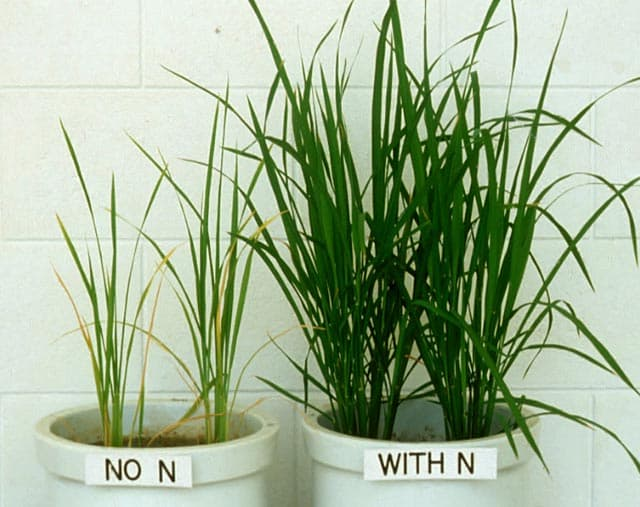
\includegraphics[scale=.37]{figures/lack-of-nitrogen.jpg}
                    \tiny\url{https://www.lgt.tw/science/2018/11/21/lack-of-nitrogen.html}
        \end{center}
    \end{frame}

    \begin{frame}{3. Der begrenzte Düngervorrat}
        \begin{minipage}{10.5cm}
            \begin{itemize}
                \item Gebiete, in denen zahlreich geerntet wurde, beginnen, den Stickstoff im Boden zu verlieren
                \item Ende 19. Jahrhundert wuchs die Weltbevölkerung exponentiell
                \item obwohl Atmosphäre 78\% aus Stickstoff besteht, können Pflanzen diese Moleküle nicht verwenden
                \item Stickstoff wird von einer Dreifachbindung zusammengehalten
            \end{itemize}
        \end{minipage}
        \hspace{.25cm}
        \begin{minipage}{1cm}
            \chemfig[
                atom style={scale=2}
                ]{[:30]\color{d_blue}{N}~\color{d_blue}{N}}
        \end{minipage}
    \end{frame}

    \begin{frame}{3. Der begrenzte Düngervorrat}
            \begin{itemize}
                \item Pflanzen können Stickstoff in Form von Ammonium ($NH{_4}{^+}$) oder Nitrat ($NO{_3}{^-}$)-Ionen aufnehmen
                \item Stickstoff-Fixierung: Ionen entstehen in der Natur durch hohen Energieaufwand
                \begin{itemize}
                    \item[$\rightarrow$] Beispiele: Blitze, Bakterien (Nitrogenase)
                \end{itemize}
                \item natürliche Vorgänge waren jedoch zu ineffizient für die Stickstoffversorgung
                \item[\alert{$\rightarrow$}] \alert{ein chemischer Vorgang zur Synthese von verwendbaren Stickstoff musste entwickelt werden}
            \end{itemize}
    \end{frame}

    \section{\textbf{4.} Das Haber-Bosch-Verfahren}

    \subsection{\textbf{4.1} Der Katalysator}

    \begin{frame}{4.1 Der Katalysator}
        Für die Ammoniaksynthese müssen Stickstoff und Wasserstoff zusammen reagieren. 
        $$N_{2(g)}\hspace{.15cm} +\hspace{.15cm} 3H_{2(g)}\hspace{.25cm} \rightleftharpoons\hspace{.25cm} 2NH_{3(g)}$$
        \vspace{-.75cm}
        \begin{itemize}
            \item Reaktion kann nicht bei Standardbedingungen ablaufen
            \item ein Katalysator wird eingesetzt: Magnetit bzw. Ferrit (Ein Gemisch aus $FeO$ und $Fe_2O_3$)
            \item durch Adsorption der Moleküle an das Ferrit (Anlagerung an der Oberfläche) werden Stickstoff und Wasserstoff leichter gespalten (Dissoziation)
            \item Stickstoff und Wasserstoff reagieren schrittweise zu Ammoniak, das schließlich desorbiert (Abtrennung von der Oberfläche)
            \item Reaktion läuft mit höherer Temperatur schneller ab
        \end{itemize}
    \end{frame}
    
    \subsection{\textbf{4.2} Die Rolle des kleinsten Zwangs}

    \begin{frame}{4.2 Die Rolle des kleinsten Zwangs - Temperatur und Druck}
        Schauen wir uns die chemische Gleichung genauer an...
        $$N_{2(g)}\hspace{.15cm} +\hspace{.15cm} 3H_{2(g)}\hspace{.25cm} \rightleftharpoons\hspace{.25cm} 2NH_{3(g)}\hspace{.25cm}|\hspace{.1cm}exotherm$$
        $\rightarrow$ Ziel ist es, die Produktseite zu begünstigen.\newline
        \begin{minipage}{6.75cm}
            \vspace{.5cm}
            \textbf{Temperatur}
            \begin{itemize}
                \item Reaktion läuft exotherm ab
                \item bei Temperaturerniedrigung wird Produktseite begünstigt
                \item Idealtemperatur für Synthese liegt bei ca. 500°C wegen Katalysator
            \end{itemize}
        \end{minipage}
        \begin{minipage}{6.75cm}
            \vspace{.5cm}
            \textbf{Druck}
            \begin{itemize}
                \item Auf der Eduktseite befinden sich mehr Teilchen
                \item Durch der Druckerhöhung wird die Produktseite begünstigt
                \item 300 Bar als Idealdruck
            \end{itemize}
        \end{minipage}
    \end{frame}
    
    \subsection{\textbf{4.3} Die industrielle Umsetzung}

    \begin{frame}{4.3 Die industrielle Umsetzung}\hspace{-1cm}
        \begin{minipage}{10cm}
            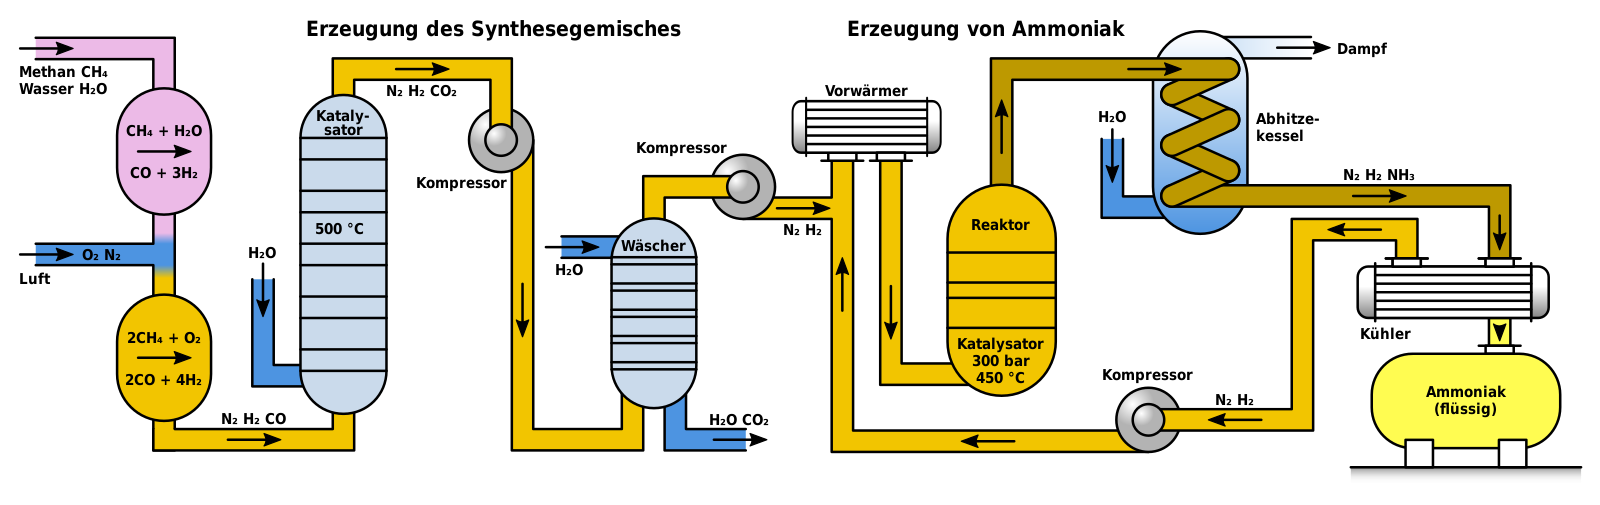
\includegraphics[scale=.28]{figures/Haber-Bosch-Process.png}
        \tiny\url{https://commons.wikimedia.org/wiki/File:Haber-Bosch.svg}
        \end{minipage}
    \end{frame}        

    \section{\textbf{5.} Fritz Haber und Carl Bosch}
    
    \begin{frame}{5.1 Carl Bosch}    
        \begin{minipage}{10cm}
            \begin{itemize}
                \item geboren 1874 in Köln, gestorben 1940 in Heidelberg
                \item Ingenieur bei BASF
                \item brachte das Verfahren auf die industrielle Ebene
                \begin{itemize}
                    \item[$\rightarrow$] entwickelte den ersten Teil des Haber-Bosch-Verfahrens für die Erzeugung des Synthesegemisches                
                \end{itemize}
                \item spielte eine wichtige Rolle beim Bau der ersten Fabrik in Ludwigshafen-Oppau
            \end{itemize}    
        \end{minipage}
            \begin{minipage}{3.5cm}
                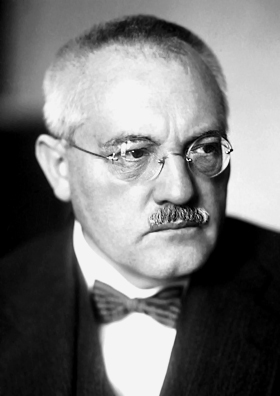
\includegraphics[scale=.42]{figures/Carl_Bosch.jpg}
                \tiny\color{gray}\url{https://de.wikipedia.org/wiki/Carl_Bosch}
            \end{minipage}
    \end{frame}
   

    \begin{frame}{5.2 Fritz Haber}
        \begin{minipage}{4.25cm}
            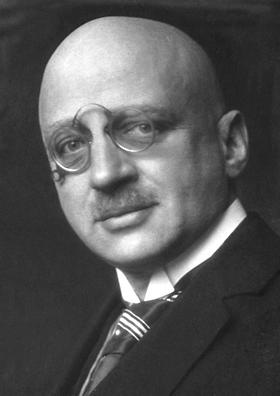
\includegraphics[scale=.42]{figures/Fritz_Haber.png}
            \tiny\color{gray}\url{https://de.wikipedia.org/wiki/Fritz_Haber}
        \end{minipage}
        \begin{minipage}{9.25cm}
            \begin{itemize}
                \item geboren 1868 in Breslau, Polen; gestorben 1934 in Basel
                \item war auf die synthetische Herstellung on nitratbasierte Sprengstoffe ausgerichtet
                \item durch seine Entdeckung als nationaler Held angesehen
                \begin{itemize}
                    \item[$\rightarrow$] wurde Leiter des Kaiser-Wilhelm-Institut in Berlin
                    \item[$\rightarrow$] erhielt den Nobelpreis für Chemie in 1918, jedoch war Preisübergabe sehr umstritten
                \end{itemize}
            \end{itemize}
        \end{minipage}
    \end{frame}

    \begin{frame}{5.2 Fritz Haber - 1. Weltkrieg}
        \begin{minipage}{6cm}
            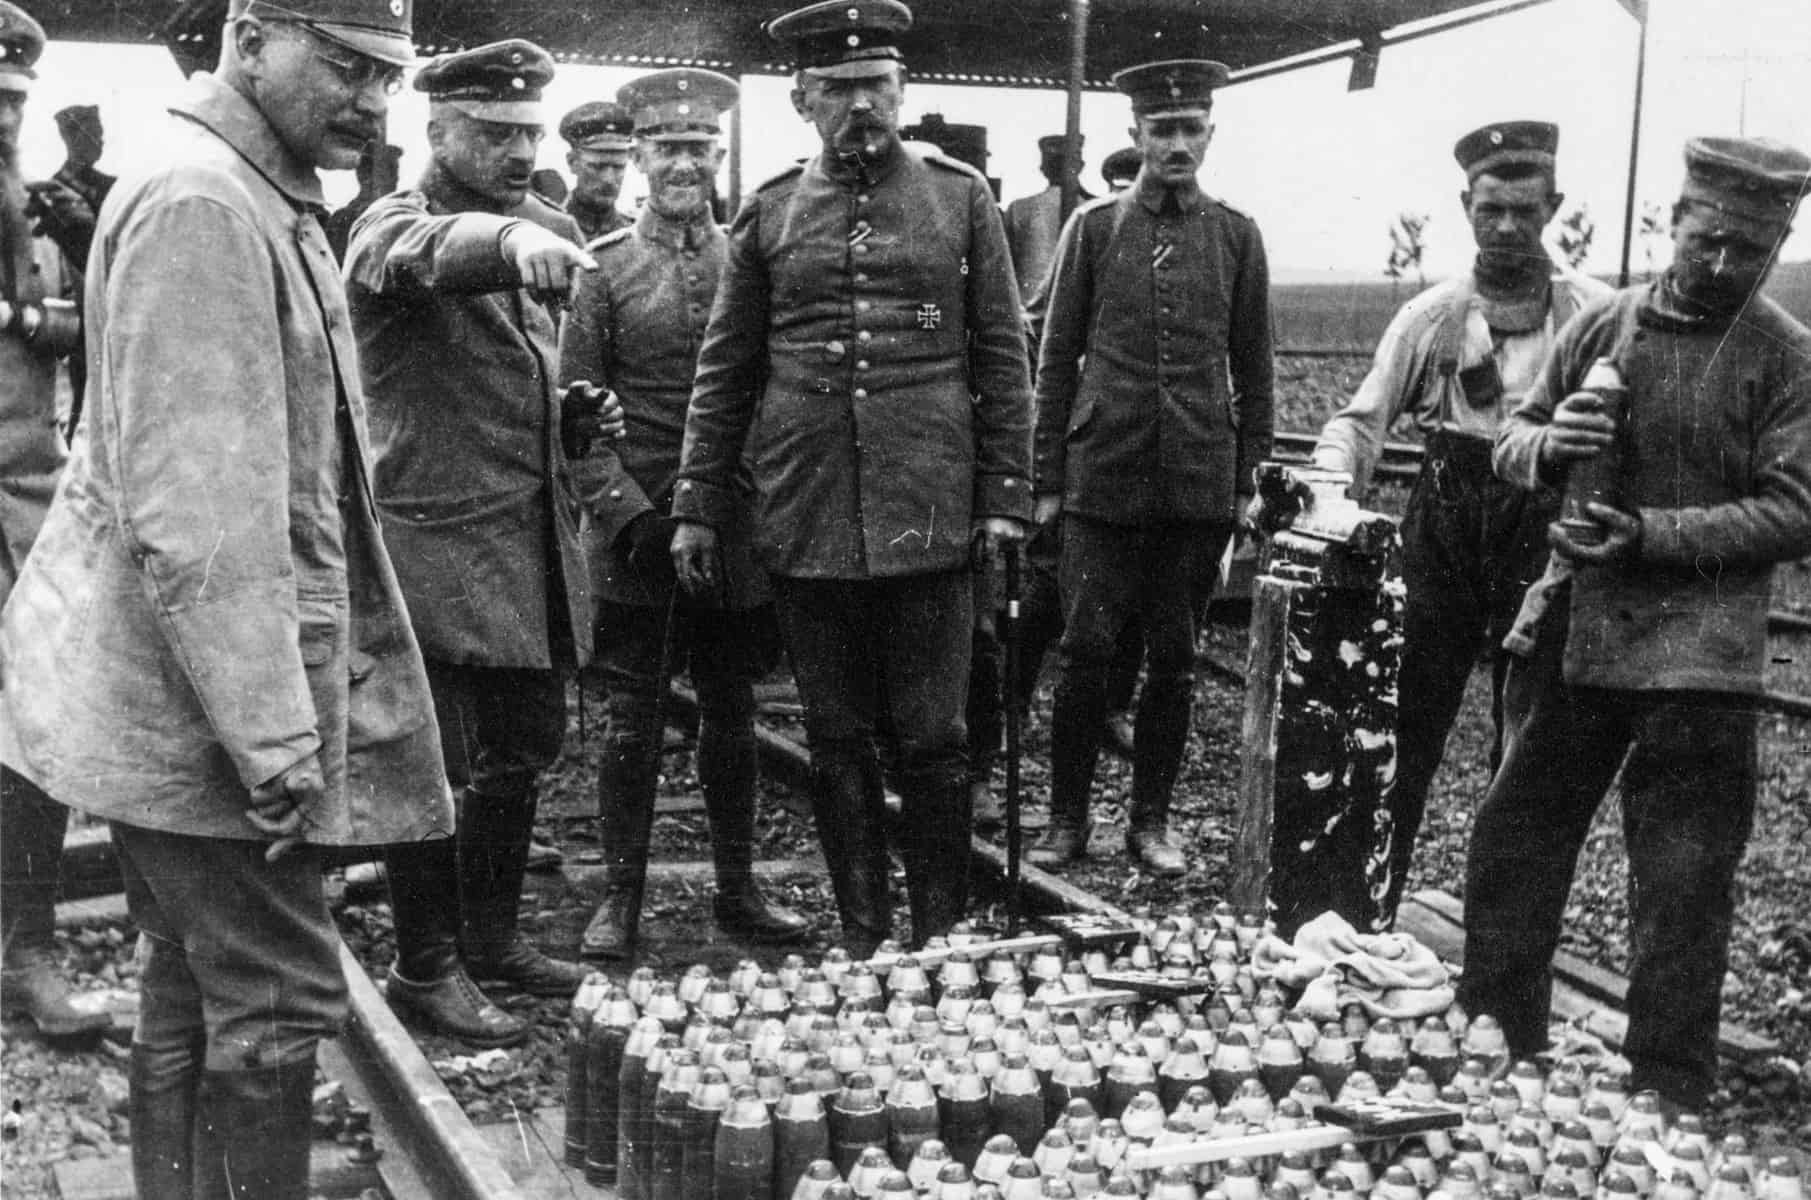
\includegraphics[scale=.09]{figures/HaberChlorine.jpg}
            \tiny\color{gray}\url{https://historycollection.com/fritz-haber-the-monster-who-made-the-modern-world-possible/}
        \end{minipage}
        \begin{minipage}{7.75cm}
            \begin{itemize}
                \item Trotz Hass gegen Menschen jüdischer Abstammung, war Haber ein deutscher Patriot
                \item war stark im 1. Weltkrieg beteiligt und für die Herstellung von chemischen Waffen wie Chlor- und Senfgas zuständig
            \end{itemize}
        \end{minipage}
    \end{frame}
    
    \begin{frame}{5.2 Fritz Haber}
        \begin{minipage}{9.5cm}
            \begin{itemize}
                \item stand nach der Machtübergreifung Hitlers unter politischen Druck
                \item folgend trat er von der Leitung des Kaiser-Wilhelm-Instituts zurück
                \item starb am 29. Januar 1934 in Basel, nachdem er von der Universität von Cambridge aufgenommen wurde
                \item nach seinem Tod haben deutsche Chemiker sein bereits hergestelltes Pestizid Zyklon-A umgeändert (Warngeruch wurde entfernt)
                \begin{itemize}
                    \item[$\rightarrow$] Entwicklung von Zyklon-B, das in Konzentrationslagern verwendet wurde
                \end{itemize}
            \end{itemize}
        \end{minipage}
        \hspace{.25cm}
        \begin{minipage}{1cm}
            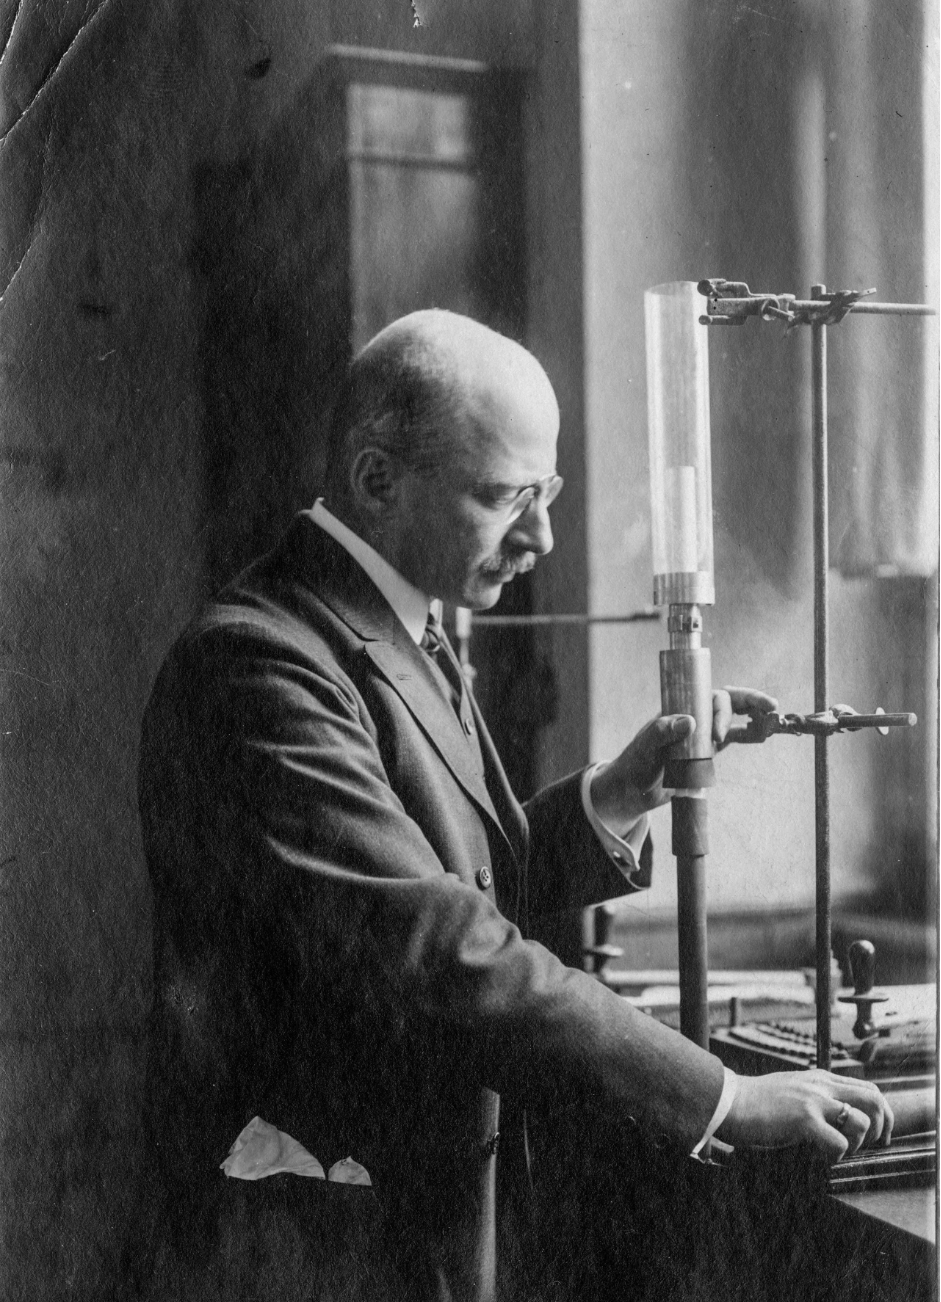
\includegraphics[scale=.25]{figures/Fritz_Haber_Ammoniakapp.png}
        \end{minipage}
    \end{frame}

    \section{\textbf{6.} Auswirkungen auf die heutige Welt}

    \begin{frame}{6. Auswirkungen auf die heutige Welt}
            \begin{center}
                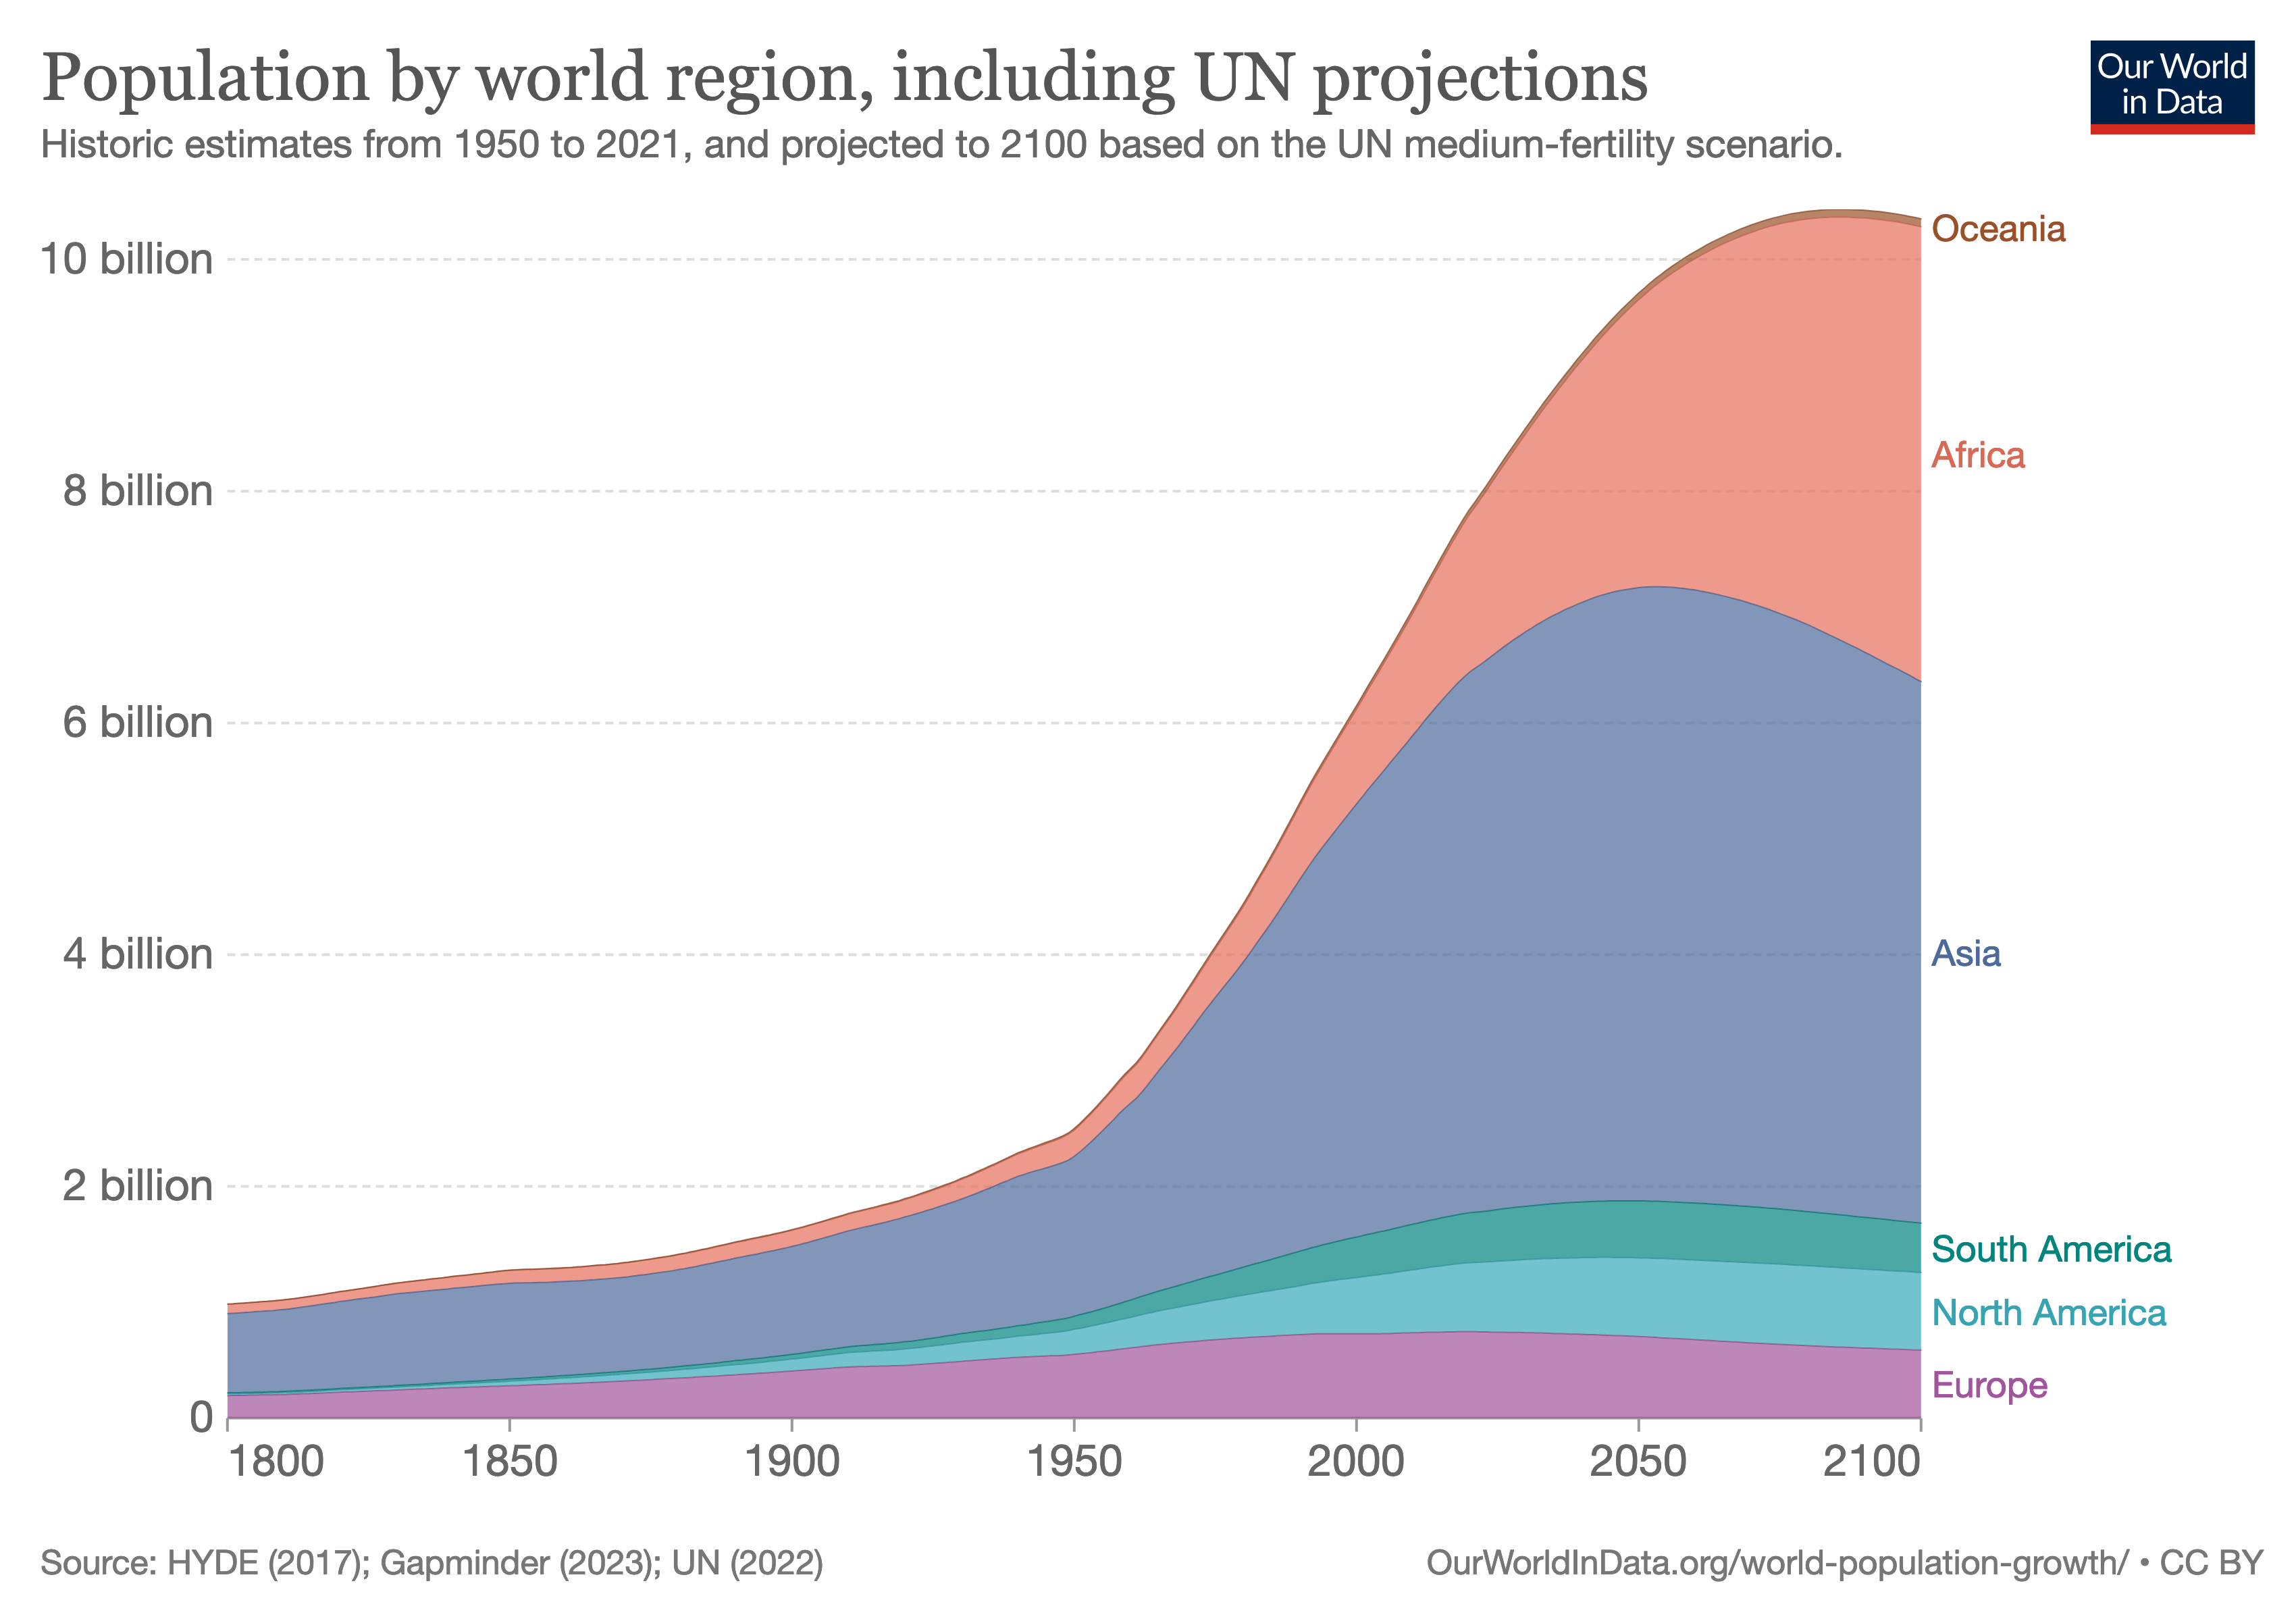
\includegraphics[scale=.1]{figures/world_pop.png}
            \end{center}
    \end{frame}

    \begin{frame}{6. Auswirkungen auf die heutige Welt}
        \begin{minipage}{6cm}
            \textbf{Positive Aspekte}
            \begin{itemize}
                \item weniger Länder wurden von der südamerikanischen Guano-Versorgung abhängig
                \item die Erde kann jetzt 4 Milliarden Menschen mehr aufnehmen früher
                \item du könntest sogar dein Leben Habers Erfindung verdanken!
            \end{itemize}    
        \end{minipage} 
        \hspace{.25cm}  
        \begin{minipage}{7cm}
            \textbf{Negative Aspekte}
            \begin{itemize}
                \item stickstoffbasierte Sprengstoffindustrie ist seit dem Haber-Bosch-Verfahren in Gang gekommen
                \item Überproduktion von Ammoniak: Ammoniak gelangt in Flüssen und Meeren
                \begin{itemize}
                    \item[$\rightarrow$] übermäßige Algenbewachsung, die zum Überverbrauch von Sauerstoff führt (Entstehung von "dead zones")
                \end{itemize}
            \end{itemize}
        \end{minipage} 
    \end{frame}

    \section{\textbf{7.} Fazit}

    \begin{frame}{7. Fazit}
        \begin{itemize}
            \item ``Turning air into bread'' - obwohl er Deutschland auf den nächsten Krieg vorbereiten wollte, löste er am Ende eines der größten Probleme seiner Zeit
            \begin{itemize}
                \item[$\rightarrow$] Fritz Haber lässt sich bis heute noch schwierig als Held oder Schurke einordnen
            \end{itemize} 
            \item die Ammoniaksynthese ermöglichte die Herstellung großer Mengen an Munition für die deutsche Armee
            \item eine Alternative für die nachhaltige Herstellung von Ammoniak bzw. des Synthesegemisches ist noch zu finden
            \item der wichtigste Prozess zur Schaffung einer modernen Welt wie wir sie kennen
        \end{itemize}
    \end{frame}

    \begin{frame}{Vielen Dank für eure Aufmerksamkeit!}
        \large\textbf{Habt ihr noch Fragen?}
    \end{frame}
    
    \begin{frame}{8. Quellen (Stand: 22. März 2023)}
        \tiny\begin{itemize}
            \item \url{https://www.youtube.com/watch?v=EvknN89JoWo}
            \item \url{https://www.worldatlas.com/articles/what-is-guano.html}
            \item \url{https://www.science.org/content/article/how-bird-poop-helps-cool-arctic}
            \item \url{https://utopia.de/ratgeber/guano-duenger-besonderheiten-anwendung-und-nachteile/} 
            \item \url{https://99percentinvisible.org/episode/guano-mania/}
            \item \url{https://rootsofprogress.org/turning-air-into-bread}
            \item \url{https://www.dhm.de/lemo/biografie/fritz-haber}
            \item \url{https://www.chemie.de/lexikon/Ammoniak.html}
            \item \url{https://www.basf.com/global/de/media/events/2019/full-year-results/photos-pk.fragment.html/overview_copy_copy_c$/global/press-photos/de/photos/2019/02/annual-press-conference/10_5114_Ammonia_plant_at_Ludwigshafen_site.jpg.html}
            \item \url{http://daten.didaktikchemie.uni-bayreuth.de/umat/haber/archiv/haber.htm}
            \item \url{https://historycollection.com/fritz-haber-the-monster-who-made-the-modern-world-possible/}
            \item \url{https://chemicalengineeringworld.com/nfpa-national-fire-protection-association/}
            \item \url{https://www.lgt.tw/science/2018/11/21/lack-of-nitrogen.html}
            \item \url{https://www.nagwa.com/en/videos/590147806076/}
            \item \url{https://www.weforum.org/agenda/2021/12/world-population-history}
            \item \url{https://www.discovermagazine.com/the-sciences/6-times-we-tried-to-extract-gold-from-seawater}
            \item \url{https://www.youtube.com/watch?v=tdEE5uvFhOM}
            \item \url{https://www.wired.com/2015/10/nobel-committee-hasnt-always-picked-right-winners/}
            \item The Alchemy of Air. A Jewish Genius, a Doomed Tycoon, and the Scientific Discovery That Fed the World but Fueled the Rise of Hitler, Thomas Hager
            \item Fokus Chemie · Gesamtband Sekundarstufe II
        \end{itemize}           
    \end{frame}

\end{document}